\section{Modelling}
\subsection{Choosing a Method}
\begin{frame}\frametitle{Choosing the appropriate method}
It is essential, therefore, that you can answer the following questions:
\begin{itemize}
\item Which of your variables is the response variable?
\item Which are the explanatory variables?
\item Are the explanatory variables continuous or categorical, or a mixture of both?
\item What kind of response variable do you have: is it a continuous measurement, a count, a proportion, a time at death, or a category?
\end{itemize}
%These simple keys will lead you to the appropriate statistical method:
%A data frame with 500 observations on the following 8 variables. 
%From: Michael Hills and Bianca De Stavola (2002). A Short Introduction
%     to Stata 8 for Biostatistics, Timberlake Consultants Ltd <URL:
%     http://www.timberlake.co.uk>
\end{frame}

\begin{frame}\frametitle{Choosing the appropriate method}
\begin{center}\footnotesize
    \rowcolors[]{1}{gray!10}{gray!30}
  \begin{tabular}{@{} >{\ttfamily}l l} 
    \rowcolor{gray!40}
Explanatory Variables are & \\
all  continuous                  & Regression                     \\ 
all categorical & Analysis of variance (ANOVA)   \\
both continuous and categorical & Analysis of covariance (ANCOVA)\\
  \end{tabular}
\end{center}
\end{frame}

\begin{frame}\frametitle{Choosing the appropriate method}
\begin{center}
    \rowcolors[]{1}{gray!10}{gray!30}
  \begin{tabular}{@{} >{\ttfamily}l l} 
    \rowcolor{gray!40}
Response Variables & \\
(a) Continuous   & Normal regression, ANOVA or ANCOVA\\
(b) Proportion   & Logistic regression               \\
(c) Count        & Log-linear models                 \\
(d) Binary       & Binary logistic analysis          \\
(e) Time at death& Survival analysis                 \\
  \end{tabular}
\end{center}
The best model is the model that produces the \textbf{least unexplained variation} (the minimal residual
deviance), subject to the constraint that \textbf{all the parameters} in the model \textbf{should be statistically
significant}.
\end{frame}

\begin{frame}\frametitle{Choosing the appropriate method}
  \begin{itemize}
  \item It is very important to understand that there is not \emph{one} model;
  \item there will be a large number of different, more or less plausible models that   might be fitted to any given set of data. 
  \end{itemize}
\end{frame}

\begin{frame}\frametitle{Maximum Likelihood}
We define \emph{best} in terms of maximum likelihood.
\begin{itemize}
\item given the data,                                                                
\item and given our choice of model,                                                 
\item what values of the parameters of that model make the observed data most likely?
\end{itemize}
We judge the model on the basis how likely the data would be if the model were correct. 
\end{frame}

\begin{frame}\frametitle{Ockham's Razor}
The principle is attributed to William of Ockham, who insisted that, given a set of equally good explanations
for a given phenomenon, the correct explanation is the simplest explanation. The most useful statement of the principle for scientists is when you have two competing theories which make exactly the same predictions, the one that is simpler is the better.
\end{frame}

\begin{frame}\frametitle{Ockham's Razor}
For statistical modelling, the principle of
parsimony means that:
\begin{itemize}
\item models should have as few parameters as possible;
\item linear models should be preferred to non-linear models;
\item experiments relying on few assumptions should be preferred to those relying on many;
\item models should be pared down until they are minimal adequate;
\item simple explanations should be preferred to complex explanations.
\end{itemize}
\end{frame}

\subsection{Types of Models}
\begin{frame}\frametitle{Types of Models}
Fitting models to data is the central function of R. There are no fixed rules and no absolutes. The object is to determine a minimal adequate model from a large set of potential models. For this reason we looking at the following types of models: 
\begin{itemize}
\item the null model;
\item the minimal adequate model;
\item the maximal model; and
\item the saturated model.
\end{itemize}
\end{frame}

\begin{frame}\frametitle{The Null model}
\begin{columns}
\begin{column}{0.6\textwidth}
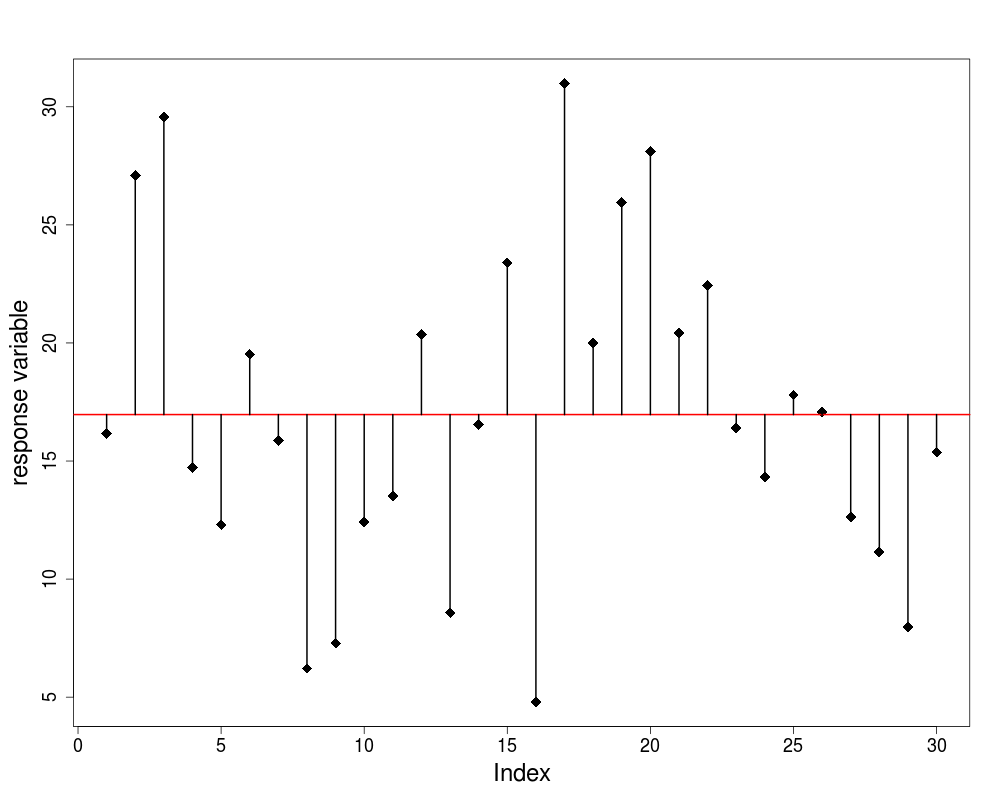
\includegraphics[width=6.5cm]{img/nullmodel.png}
\end{column}
\begin{column}{0.4\textwidth}
\begin{itemize}
\item Just one parameter, the overall mean $\bar{y}$
\item Fit: none; $SSE = SSY$
\item Degrees of freedom: $n-1$
\item Explanatory power of the model: none
\end{itemize}
\end{column}
\end{columns}
\end{frame}

\begin{frame}\frametitle{Adding Information}
Minimal adequate model:
\begin{columns}
\begin{column}{0.6\textwidth}
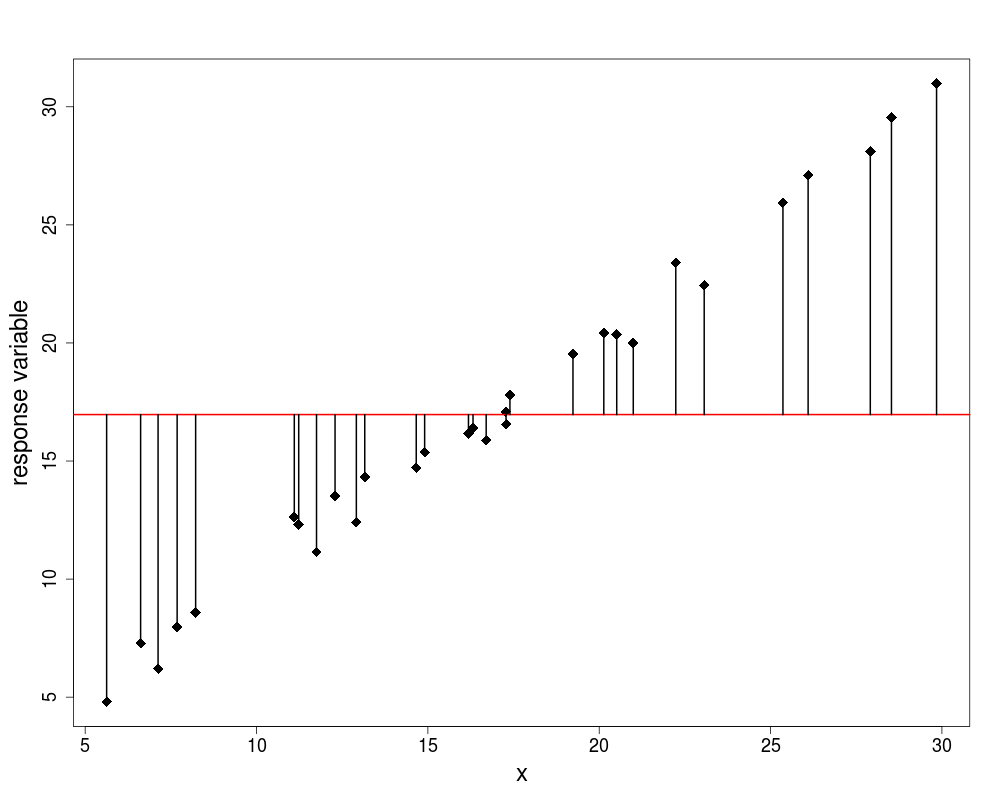
\includegraphics[width=6.5cm]{img/minimalmodel.png}
\end{column}
\begin{column}{0.4\textwidth}
\begin{itemize}
\item model with $0 \le p' \le p$ parameters
\item Fit: less than the maximal model, but not significantly so
\item Degrees of freedom: $n-p'-1$
\item Explanatory power of the model: $r^2 = \frac{SSR}{SSY}$    
\end{itemize}
\end{column}
\end{columns}
\end{frame}

\begin{frame}\frametitle{Adding Information}
Minimal adequate model:
\begin{columns}
\begin{column}{0.6\textwidth}
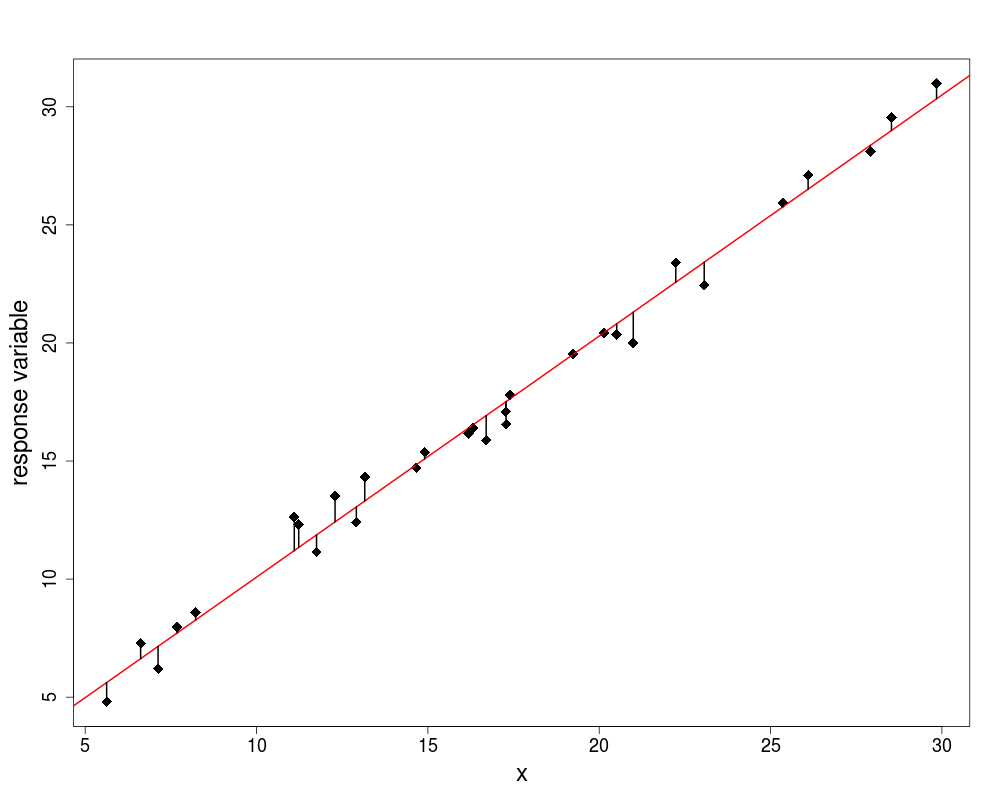
\includegraphics[width=6.5cm]{img/minimalmodel2.png}
\end{column}
\begin{column}{0.4\textwidth}
\begin{itemize}
\item model with $0 \le p' \le p$ parameters
\item Fit: less than the maximal model, but not significantly so
\item Degrees of freedom: $n-p'-1$
\item Explanatory power of the model: $r^2 = \frac{SSA}{SSY}$    
\end{itemize}
\end{column}
\end{columns}
\end{frame}

\begin{frame}\frametitle{Saturated/Maximal Model}
\begin{columns}[t]
\begin{column}{0.5\textwidth}
saturated model
\begin{itemize}
\item One parameter for every data point
\item Fit: perfect
\item Degrees of freedom: none
\item Explanatory power of the model: none
\end{itemize}
\end{column}
\begin{column}{0.5\textwidth}
maximal model
\begin{itemize}
\item Contains all $p$ factors, interactions and covariates that
\item Degrees of freedom: $n-p-1$
\item Explanatory power of the model: it depends
\end{itemize}
\end{column}
\end{columns}
\end{frame}

\begin{frame}\frametitle{How to choose...}
\begin{itemize}
\item models are representations of reality that should be both accurate and convenient
\item it is impossible to maximize a model’s realism, generality and holism simultaneously
\item the principle of parsimony is a vital tool in helping to choose one model over another
\item only include an explanatory variable in a model if it significantly improved the fit of the model (or if there other strong reasons)
\item the fact that we went to the trouble of measuring something does not mean we have to have it in our model
\end{itemize}
\end{frame}

\section{ANOVA}
\begin{frame}\frametitle{ANOVA}
  \begin{itemize}
  \item a technique we use when all explanatory variables are categorical (factor)
  \item if there is one factor with three or more levels we use one-way ANOVA (only two levels: t-test should be preferred, would give exactly the same answer since with 2 levels $F=t^2$)
  \item for more factors there there is two-way, three-way anova 
  \item central idea is to compare two or more means by comparing variances
  \end{itemize}
\end{frame}

\subsection{Data}
\begin{frame}[fragile]\frametitle{The Garden Data}
A data frame with 14 observations on 2 variables. 
\begin{center}
\rowcolors{1}{gray!10}{gray!30}
\begin{tabular}{@{} >{\ttfamily}r l}
  ozone: & athmospheric ozone concentration               \\
  garden: & garden id                              \\
\end{tabular}

\vspace*{1cm}

\begin{table}[ht]
\small
\centering
\begin{tabular}{rllllllllllllll}
  \hline
 & 1 & 2 & 3 & 4 & 5 & 6 & 7 & 8 & 9 & 10 & 11 & 12 & 13 & 14 \\ 
  \hline
ozone &  9 &  7 &  6 &  8 &  5 & 11 &  9 & 11 &  9 &  6 & 10 &  8 &  8 & 12 \\ 
  garden & a & a & a & b & a & b & b & b & b & a & b & a & a & b \\ 
   \hline
\end{tabular}
\end{table}
\end{center}
From: Michael Crawley, The R-Book

\end{frame}

\subsection{Sums of Squares}
\begin{frame}\frametitle{Total Sum of Squares}
\tikzstyle{na} = [baseline=-.5ex]
  \begin{itemize}
  \item  we plot the values in order they are measured
  \end{itemize}
\begin{center}
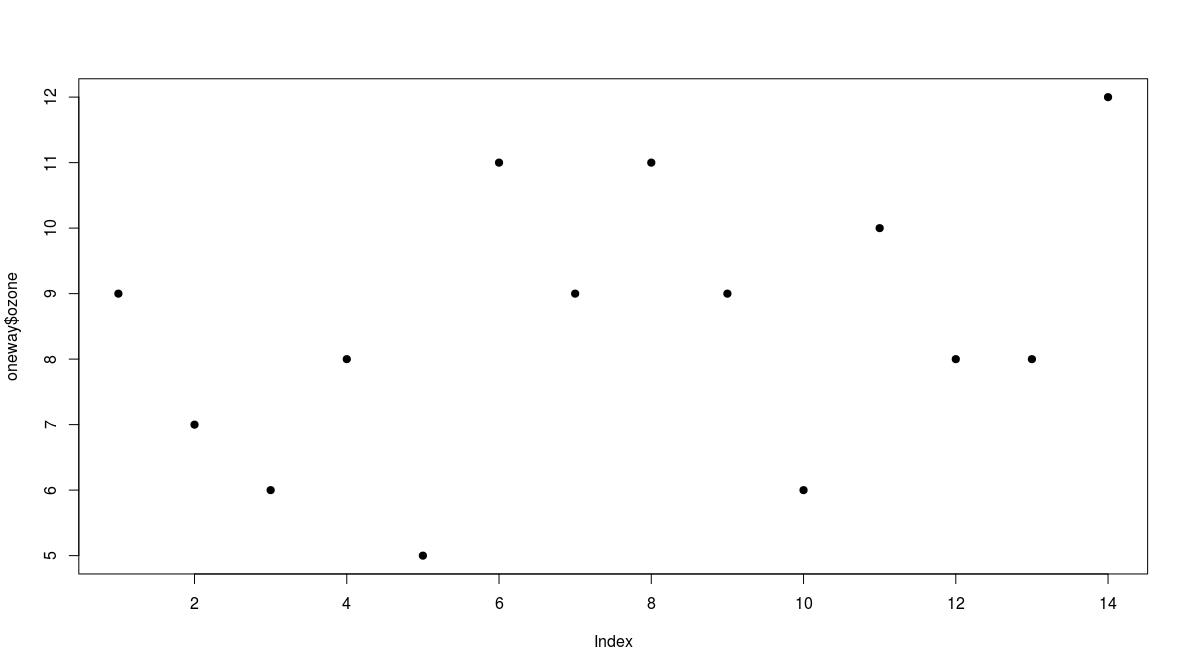
\includegraphics[width=11cm]{TSS1.png}
\end{center}
\end{frame}

\begin{frame}\frametitle{Total Sum of Squares}
  \begin{itemize}
  \item  there is a lot of scatter, indicating that the variance in ozone is large
  \item to get a feel for the overall variance we plot the overall mean (8.5) and indicate each of the residuals by a vertical line
  \end{itemize}
\end{frame}

\begin{frame}\frametitle{Total Sum of Squares}
\begin{center}
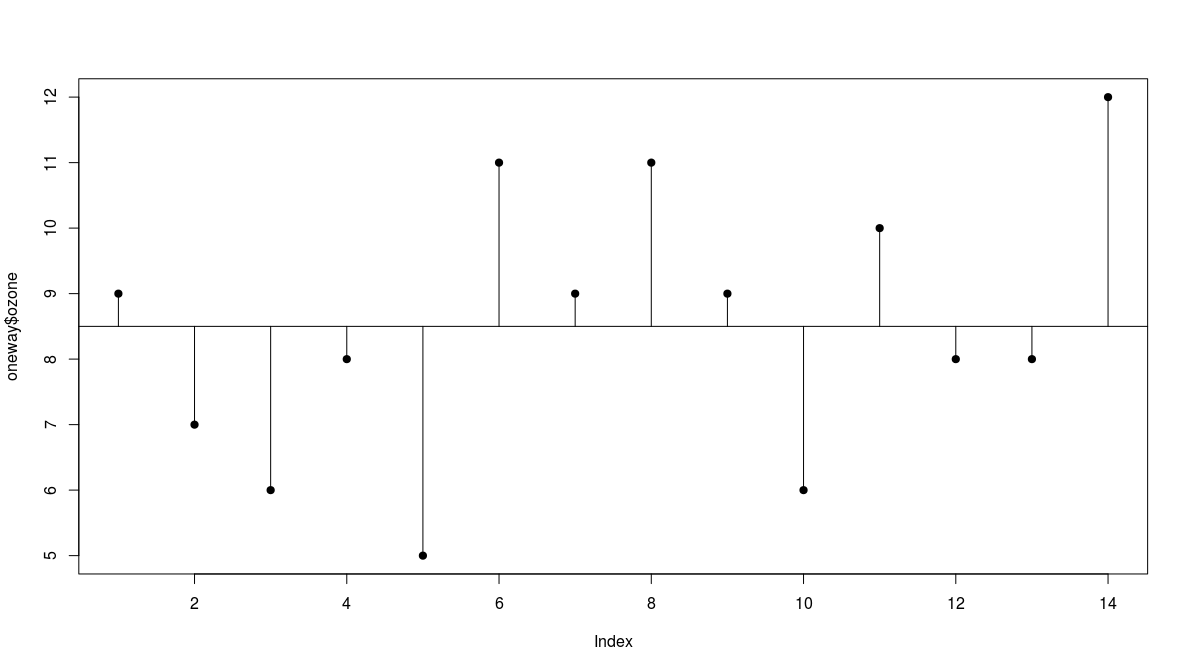
\includegraphics[width=11cm]{img/TSS.png}
\end{center}
\end{frame}

\begin{frame}\frametitle{Total Sum of Squares}
  \begin{itemize}
  \item we refer to this overall variation as the \emph{total sum of squares, SSY or TSS} 
$$ SSY = \sum(y-\bar{y})^2$$
  \end{itemize}
\end{frame}

\begin{frame}\frametitle{Total Sum of Squares}
  \begin{itemize}
  \item in this case $$SSY = 55.5$$
  \end{itemize}
   \tikzstyle{background grid}=[draw, black!50,step=.5cm]
        \begin{tikzpicture}
            % Put the graphic inside a node. This makes it easy to place the
            % graphic and to draw on top of it. 
            % The above right option is used to place the lower left corner
            % of the image at the (0,0) coordinate. 
            \node [inner sep=0pt,above right] 
                {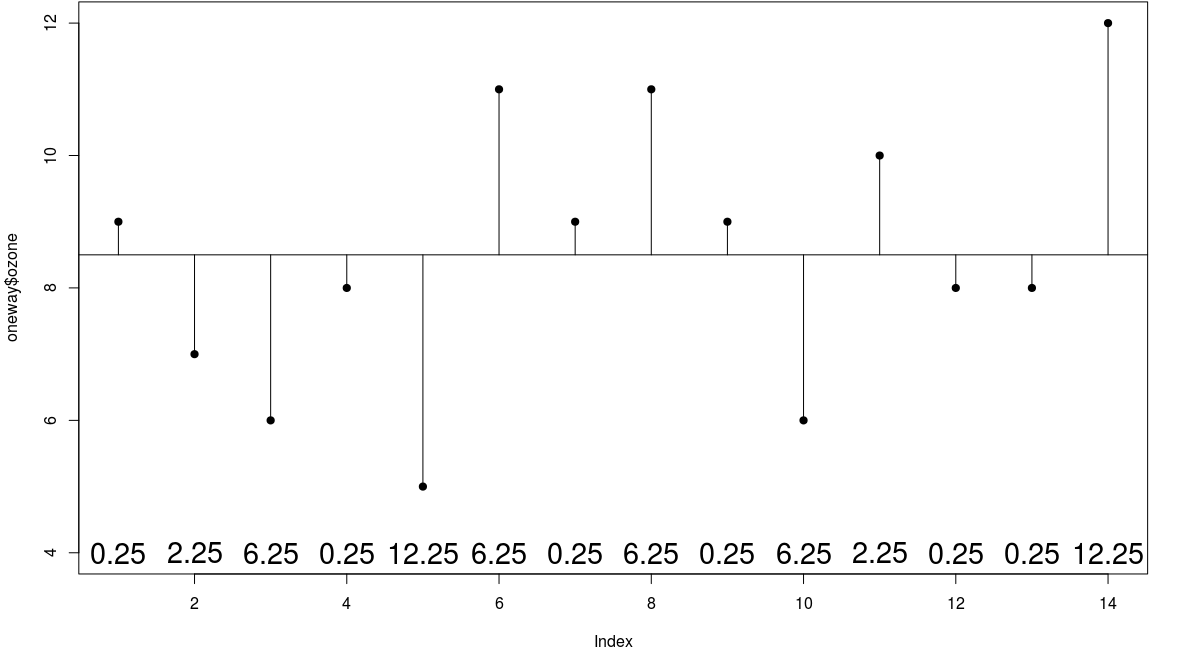
\includegraphics[width=11cm]{TSS2.png}};
            \filldraw[fill=blue!40,opacity=.5] (5.7,1.1) ellipse (5cm and 0.5cm);
%%            \fill (21.5,1.8) circle (2pt);
            % define destination coordinates
        \end{tikzpicture}
\end{frame}

\begin{frame}\frametitle{Group Means}
  \begin{itemize}
  \item now instead of fitting the overall mean, let us fit the individual garden means
  \end{itemize}
\begin{table}[ht]
\centering
\begin{tabular}{lcc}
  \hline
garden & a & b \\ 
  mean &  7 & 10 \\ 
   \hline
\end{tabular}
\end{table}
\end{frame}

\begin{frame}\frametitle{Group Means}
\tikzstyle{na} = [baseline=-.5ex]
  \begin{columns}
    \begin{column}{0.7\paperwidth}
      \begin{itemize}
      \item[]  \tikz[na] \coordinate (s-A); Garden A
      \end{itemize}
    \end{column}
    \begin{column}{0.4\paperwidth}
      \begin{itemize}
      \item[] Garden B \tikz[na] \coordinate (s-B);
      \end{itemize}
    \end{column}
  \end{columns}
%%  \tikzstyle{background grid}=[draw, black!50,step=.5cm]
        \begin{tikzpicture}
            % Put the graphic inside a node. This makes it easy to place the
            % graphic and to draw on top of it. 
            % The above right option is used to place the lower left corner
            % of the image at the (0,0) coordinate. 
            \node [inner sep=0pt,above right] 
            {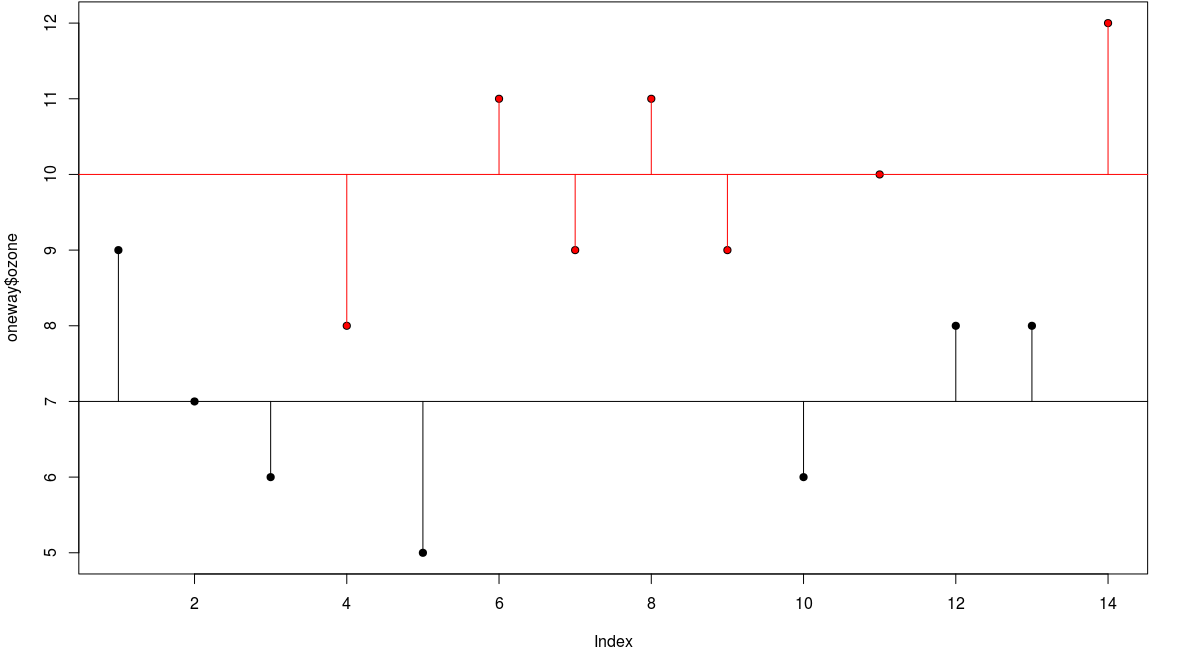
\includegraphics[width=10cm]{img/ESS.png}};
            % define destination coordinates
            \path (9.75,4.2) coordinate (B)
            (.6,2.3) coordinate (A);
        \end{tikzpicture}

% define overlays
% Note the use of the overlay option. This is required when 
% you want to access nodes in different pictures.
\begin{tikzpicture}[overlay]
        \path[->,red,thick] (s-B) edge [bend left] (B);
        \path[->,black,thick] (s-A) edge [bend right] (A);
\end{tikzpicture}

\end{frame}


\begin{frame}\frametitle{Group Means}
  \begin{itemize}
  \item now we see that the mean ozone concentration is substantially higher in garden B
  \item the aim of ANOVA is to determine 
    \begin{itemize}
    \item whether it is significantly higher \emph{or}
    \item whether this kind of difference could come by chance alone
    \end{itemize}
  \end{itemize}
\end{frame}

\begin{frame}\frametitle{Error Sum of Squares}
\emph{ When the means are significantly different then the sum of squares computed from the individual garden means will be smaller than the sum of squares computed from the overall mean. }
  \begin{itemize}
  \item we define the new sum of squares as the \emph{error sum of squares} (error in the sense of 'residual')
$$ SSE = \sum(y_{garden A}-\bar{y}_{garden A})^2+\sum(y_{garden B}-\bar{y}_{garden B})^2$$
  \end{itemize}
\end{frame}

\begin{frame}\frametitle{Total Sum of Squares}
  \begin{itemize}
  \item in this case $$SSE = 24.0$$
  \end{itemize}
\begin{center}
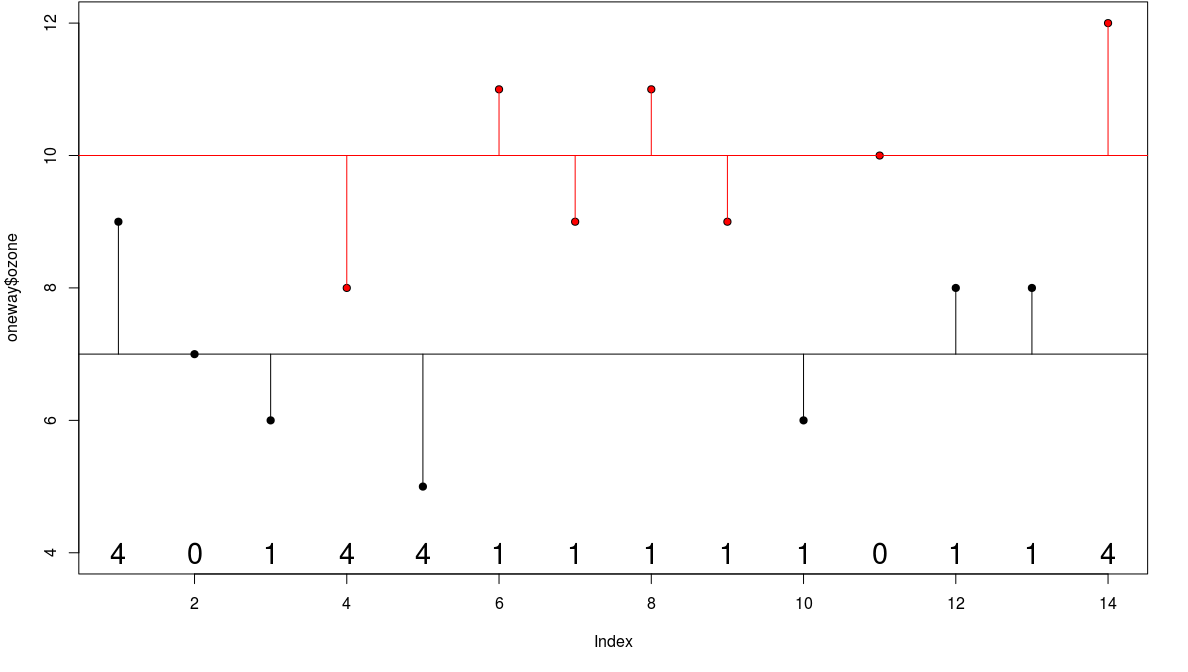
\includegraphics[width=10cm]{img/ESS2.png}
\end{center}
\end{frame}


\begin{frame}\frametitle{Treatment Sum of Squares}
\begin{itemize}
  \item then the component of the variation that is explained by the difference of the means is called the \emph{treatment sum of squares} SSA
  \item analysis of variance is based  on the notion that we break down the total sum of squares into useful and informative components
$$SSY=SSE+SSA$$ where
    \begin{itemize}
      \item SSA = explained variation
      \item SSE = unexplained variation
    \end{itemize}

  \end{itemize}
\end{frame}

\begin{frame}\frametitle{ANOVA table}
\begin{center}
\small
%% \rowcolors{1}{gray!10}{gray!30}
\begin{tabular}{@{} >{\ttfamily}l cccr}
\hline
Source & Sum of squares & Degrees of freedom & Mean square & F ratio \\
\hline
Garden &  $31.5$ & $1$ &  $31.5$ &  $15.75$\\
Error &  $24.0$ & $12$ &  $s^2=2.0$ &  \\
Total & $55.5$ & $13$ & & \\   \hline
\end{tabular}
\end{center}
\end{frame}


\begin{frame}[fragile]\frametitle{ANOVA}
  \begin{itemize}
  \item now we need to test whether an F ratio of 15.75 is large or small
  \item we can use a table or software package
  \item I use here software to calculate the cumulative probability
  \end{itemize}
\begin{verbatim}
> 1 - pf(15.75,1,12)
[1] 0.001864103
\end{verbatim}
\end{frame}

\begin{frame}\frametitle{ANOVA}
\begin{center}
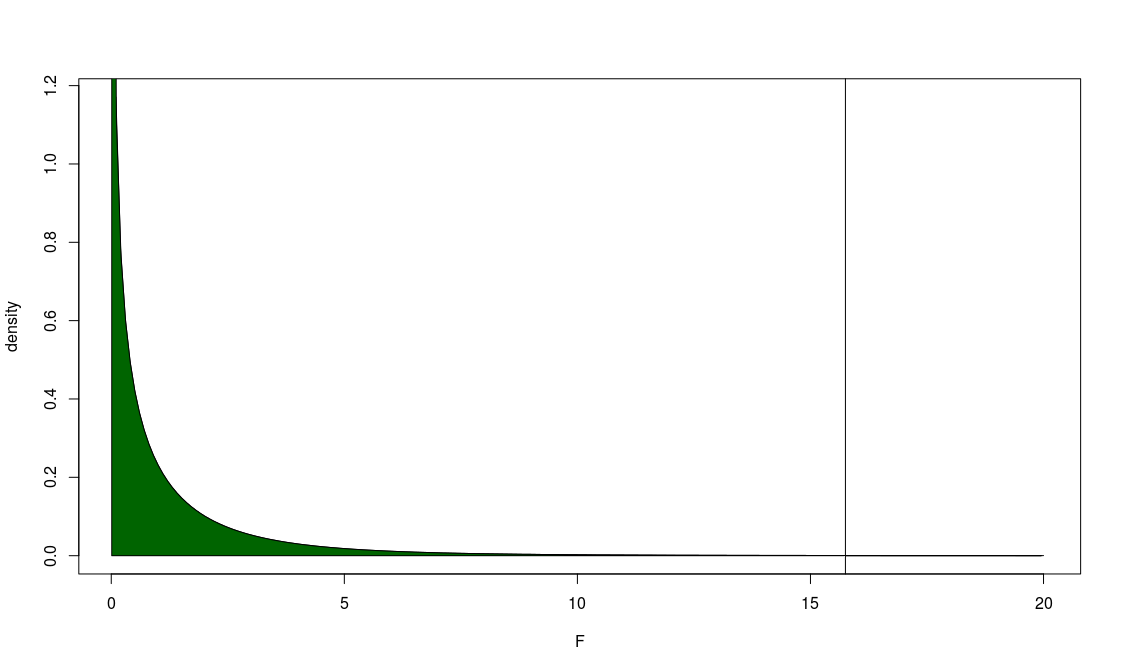
\includegraphics[width=10cm]{img/fdens.png}
\end{center}
\end{frame}


\begin{frame}[fragile]\frametitle{ANOVA in R}
  \begin{itemize}
  \item in R we use the \texttt{lm()} command and
  \item the formula syntax \texttt{a \sim  b}
  \item we assign this to an variable
 \end{itemize}
\end{frame}


\begin{frame}[fragile]\frametitle{ANOVA in R}
\begin{verbatim}
mm <- lm(ozone ~ garden, data=oneway)
mm

Call:
lm(formula = ozone ~ garden, data = oneway)

Coefficients:
(Intercept)      gardenb  
          7            3  
\end{verbatim}
\end{frame}


\begin{frame}[fragile]\frametitle{ANOVA in R}
\footnotesize
\begin{verbatim}
> summary(mm)

Call:
lm(formula = ozone ~ garden, data = oneway)

Residuals:
   Min     1Q Median     3Q    Max 
    -2     -1      0      1      2 

Coefficients:
            Estimate Std. Error t value Pr(>|t|)    
(Intercept)   7.0000     0.5345  13.096 1.82e-08 ***
gardenb       3.0000     0.7559   3.969  0.00186 ** 
---
Signif. codes:  0 ‘***’ 0.001 ‘**’ 0.01 ‘*’ 0.05 ‘.’ 0.1 ‘ ’ 1

Residual standard error: 1.414 on 12 degrees of freedom
Multiple R-squared:  0.5676,	Adjusted R-squared:  0.5315 
F-statistic: 15.75 on 1 and 12 DF,  p-value: 0.001864
\end{verbatim}
\end{frame}


\begin{frame}[fragile]\frametitle{ANOVA in R}
\footnotesize
\begin{verbatim}
> anova(mm)
Analysis of Variance Table

Response: ozone
          Df Sum Sq Mean Sq F value   Pr(>F)   
garden     1   31.5    31.5   15.75 0.001864 **
Residuals 12   24.0     2.0                    
---
Signif. codes:  0 ‘***’ 0.001 ‘**’ 0.01 ‘*’ 0.05 ‘.’ 0.1 ‘ ’ 1
\end{verbatim}
\end{frame}


\begin{frame}\frametitle{ANOVA Assumptions}
  \begin{alertblock}{Central Assumptions}
  \begin{itemize}
  \item independed, normal distributed errors
  \item equality of variances (homogeneity)
  \end{itemize}
  \end{alertblock}
\end{frame}


\begin{frame}[allowframebreaks]\frametitle{Welch ANOVA}
\begin{itemize}
\item generalization of the Welch t-test
\item tests whether the means of the outcome variables are different across the factor levels
\item assumes sufficiently large sample (greater than 10 times the number of groups in the calculation, groups of size one are to be excluded)
\item sensitive to the existence of outliers (only few are allowed)
\item the r command is \texttt{oneway.test()}
\item non-parametric alternative \texttt{kruskal.test()}
\end{itemize}
\end{frame}

\begin{frame}\frametitle{Repeated Measures ANOVA}
\tikzstyle{na} = [baseline=-.5ex]
\begin{itemize}
    \item main effect
        \tikz[na] \node[coordinate] (main) {};
    \item interaction between treatment and time
        \tikz[na]\node [coordinate] (ia) {};
\end{itemize}
  \begin{equation*}
    y_{hij} = 
    \tikz[baseline]{
      \node[fill=blue!20, anchor=base] (beta)
           {$\beta_h$};} + 
    \tikz[baseline]{
      \node[fill=red!20,anchor=base] (gamma)
           {$\gamma_{hj}$};} + 
    \tikz[baseline]{
      \node[fill=yellow!40, anchor=base] (U)
           {$U_{hi}$};} + 
    \tikz[baseline]{
      \node[fill=green!20, anchor=base] (Z)
           {$Z_{hij}$};}    
  \end{equation*}

\begin{itemize}
    \item mutually independent random effects for units
        \tikz[na]\node [coordinate] (random) {};
    \item mutually independent measurment errors
        \tikz[na]\node [coordinate] (error) {};
\end{itemize}

\begin{tikzpicture}[overlay]
        \path[->,blue,thick]<1-> (main) edge [out=0,in=90] (beta);
        \path[->,red,thick]<2-> (ia) edge [out=0,in=90] (gamma);
        \path[->,yellow,thick]<3-> (random) edge [out=0, in=-90] (U);
        \path[->,green,thick]<4-> (error) edge [out=0, in=-90] (Z);
\end{tikzpicture}

\begin{tikzpicture}[overlay]
\path[clip] (current page.north west) rectangle (current page.south east);
\path<2>[fill=black,even odd rule,path fading=fade inside]
    (beta) circle (10cm) (beta) circle (0.7cm);
\path<3>[fill=black,even odd rule,path fading=fade inside]
    (gamma) circle (10cm) (gamma) circle (0.7cm);     
\path<4>[fill=black,even odd rule,path fading=fade inside]
    (U) circle (10cm) (U) circle (0.7cm);     
\path<5>[fill=black,even odd rule,path fading=fade inside]
    (Z) circle (12cm) (Z) circle (0.7cm);     
\path<6>[fill=black,even odd rule,path fading=fade inside]
    (Z) circle (12cm) (Z) circle (11.9cm);     
\end{tikzpicture}
\end{frame}

